\section{3. Analyzing ET data}

In all previous steps, wrangling can be thought of as a condensing process, where the primary object is to remove, clean, and transform the data into a structure that is usable. However, once the data is put into tidy form, then the data must be transformed for specific visualizations and analyses. In this section, we think of \inlineR{all\_data\_cleaned} and \inlineR{all\_data\_tidy} as launching points to gain understanding of our data. 

 Here, we are creating two data frames from \inlineR{all\_data\_tidy}: \inlineR{mem\_data} in L: 405 and then \inlineR{gamm\_data} in L: 411. In general, in data wrangling, keeping as much data as possible is essential to creating a usable data frame. However, in model wrangling, it is often best to remove variables that you will not be using. This is because some models can have complications interpreting unprocessed data types. For \inlineR{mem\_data}, we start by selecting all necessary columns for the model: \inlineR{Participant.Private.ID}, \inlineR{verb\_type},\inlineR{talker}, item \inlineR{subject\_img\_file}, \inlineR{target}, log frequency of object item \inlineR{log\_SUBTLWF\_Obj}, and  \inlineR{time\_elapsed\_rounded}. \inlineR{Participant.Private.ID} is turned into a factor in L: 408. Finally, \inlineR{tidy\_quest\_data} is joined to \inlineR{mem\_data} to add questionnaire values for each participant (e.g., \inlineR{Chinese\_accent\_experience}). In addition to the \inlineR{mem\_data}, we create \inlineR{gamm\_data} by simply cloning \inlineR{mem\_data} in L: 411 and by adding a single variable needed in the GAMM models.

\lstinputlisting[style=mystyle, firstnumber=last]{scripts/chunk-All Data: Preparing for Models.R}

There are a handful of excellent papers that outline the advantages and disadvantages of different methods of eye-fixation analysis and relevant considerations for each method of analysis \parencite{Ito_Knoeferle_2022,Mirman_Dixon_Magnuson_2008,McMurray_2023,Barr_2008}. Here we continue to focus on the data wrangling process and present the data wrangling steps--and decisions--needed to carry out two of the more widely used statistical analyses: generalized linear mixed effect models or GLMM and generalized additive mixed effects models or GAMM. Both GLMMs and GAMMs require specific coding of the data before running models to get expected results. That is, each of these models start with coding the data correctly and building maximal models as justified by the design and working down to simpler models for model comparison. \parencite{Barr_Levy_Scheepers_Tily_2013}.

\subsection{GLMMs}

For GLMMs coding, start with data type conversion (L: 414-415). We then, can re-level both \inlineR{talker}(Native, Non-Native) and \inlineR{verb\_type}(Restrictive or Non-Restrictive) so that \inlineR{verb\_type}(Restrictive) and \inlineR{talker}-Native are both set as reference levels (L: 416-418).  We can then rename the contrasts to improve model output readability (L: 418-421). Lastly, in L: 423 through L: 430 we normalize the two variables \inlineR{time\_elapsed} and \inlineR{experience\_chinese}.

\lstinputlisting[style=mystyle, firstnumber=last]{scripts/chunk-GLMM: Leveling the Data.R}

GLMMs were built using the \inlineR{lme4} package \parencite{Bates2014-eq}. Looks to the target (coded as 1, 0) served as the dependent variable. The models included three fixed effects: \inlineR{verb\_type} (Restrictive or Non-Restrictive), \inlineR{talker}(Native, Non-Native) and their interaction (L: 432). All factor variables were coded with
effects coding L: 414-417. Random intercepts for \inlineR{subject\_img\_file}, \inlineR{time\_normalized}, and
\inlineR{Participant.Private.ID} were included, as were random slopes for \inlineR{talker} and \inlineR{verb\_type}, but correlations were removed after model comparison showed preference for parsimonious model over full model and simplified models with lower AIC and ANOVA comparisons (p<.001). The logit link function ("binomial") was specified in the model, equivalent to modeling logit-transformed response probability with identity link function. 

\lstinputlisting[style=mystyle, firstnumber=last]{scripts/chunk-GLMM: Main Model.R}

Results from the GLMM revealed a significant effect of  \inlineR{verbtype}-Restricting  ($\beta$ = 0.281, SE = 0.067, z = 4.192, p = .001), indicating more looks to targets for restrictive \inlineR{verb\_types} over non-restrictive \inlineR{verb\_types}, see figure \ref{fig:GLMER_base_model}. Additionally, an interaction between speaker and verb type was found ($\beta$ = -0.13737, SE = 0.05346, z = -2.570, p=.05).
\begin{figure}[H]
    \centering
    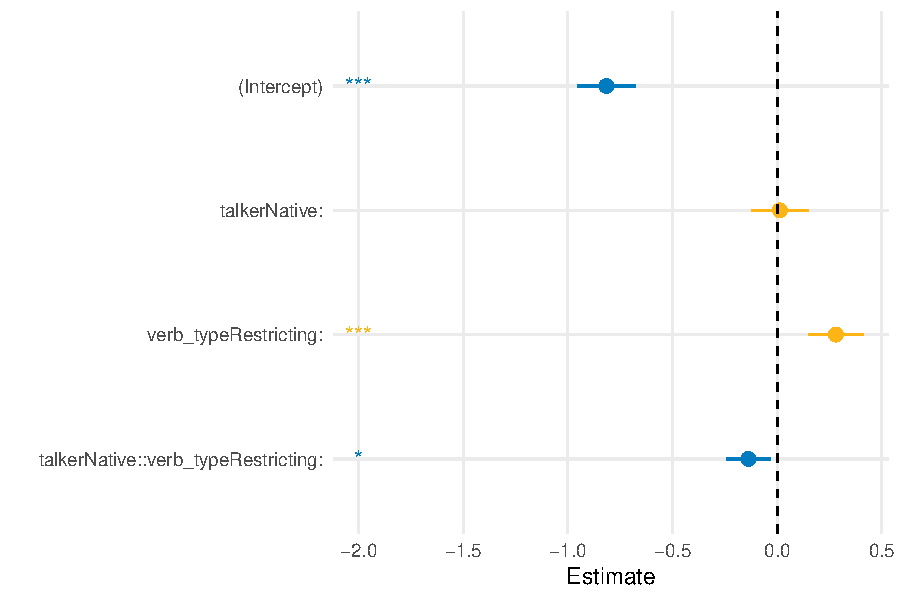
\includegraphics[width=\textwidth]{figures/GLMER_base_model.pdf}
    \caption{Model output for parsimonious model}
    \label{fig:GLMER_base_model}
\end{figure}
 Similar to the above model, an accent specific model was ran only on the data of accented speech. more here.
\begin{figure}[H]
    \centering
    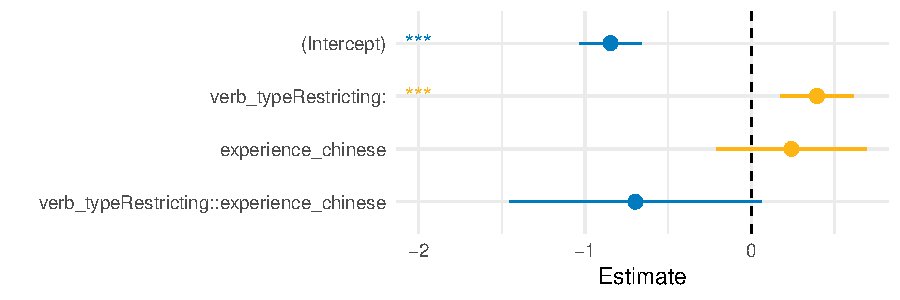
\includegraphics[width=\textwidth]{figures/GLMER_accent_model.pdf}
    \caption{place holder for real model outputs later}
    \label{fig:GLMER_accent_model}
\end{figure}

\subsection{GAMMs}
GAMMs are becoming increasingly popular as they allow the researcher to model complex time course information without the need for assumptions of linearity. Like GLMM data, GAMM data must be first coded and prepared (L: 434-446). Here, we turn variables into factors and level them at the same time (e.g., L: 442). 
\lstinputlisting[style=mystyle, firstnumber=last]{scripts/chunk-GAMM: Leveling the Data.R}
GAMM Models were built using the \inlineR{mgcv} package \parencite{mgcv_wood_2017}.
Like the GLMM, the GAMM revealed a significant effect of \inlineR{verbtype}-Restricting ($\beta$ = 0.3981, SE = 0.1293, z = 3.078, p < .005), indicating more looks to targets for restrictive \inlineR{verb\_types} over non-restrictive \inlineR{verb\_types}, see figure \ref{fig:model_gamm_effects}. Additionally, an interaction between speaker and verb type was found ($\beta$ = -0.137, SE = 0.053, z = -2.570, p=.). 
\begin{figure}[H]
    \centering
    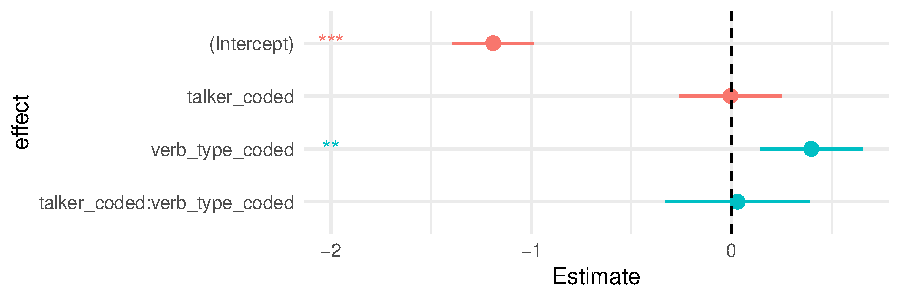
\includegraphics[width=\textwidth]{figures/model_gamm_effects.pdf}
    \caption{Model output for GAMM effects}
    \label{fig:model_gamm_effects}
\end{figure}



\subsection{Visualizing data}

For data visualization, it is often necessary to put the data into a form that is quite different than the cleaned data, either through aggregation, or by filtering, or by splitting into multiple data frames. In L: 395, we begin such an example of aggregation for visualization. Here, our goal is to create a visualization to compare looks to targets in different conditions (e.g., looks to targets for \inlineR{verb\_type} restricting vs. \inlineR{verb\_type} non-restricting sentences). In L: 397-400 we group by \inlineR{Participant.Private.ID}, condition, \inlineR{verb\_type} \inlineR{talker} and time \inlineR{time\_elapsed\_rounded} to prepare for aggregating mean looks to targets, competitors and distractors. L: 400 is created as a raw count for the calculation of empirical logits in L: 402-403.

\lstinputlisting[style=mystyle, firstnumber=last]{scripts/chunk-All Data: Preparing for Visualization.R}

For \inlineR{ggplot()} visualizations, see \inlineR{AOW\_r\_work\_flow.rmd}. We observed nearly identical time course of predictive processing, see figure \ref{fig:smooth}, in which restricted sentences resulted in earlier looks to the target object than nonrestrictive sentences. Further, this effect is even partially reduced in accented speech in a similar manner to \textcite{Porretta_et_al_2020}. 

\begin{figure}[h]
    \centering
    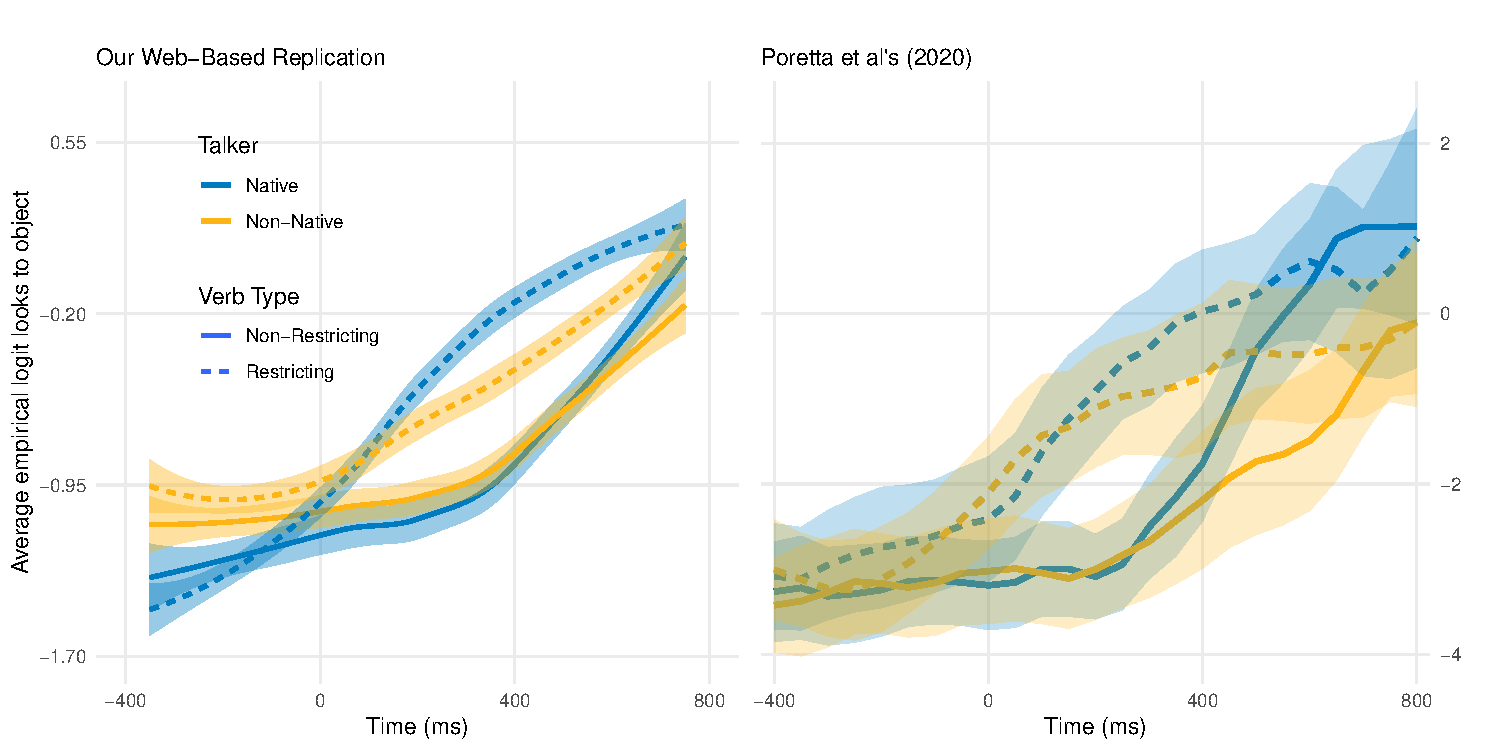
\includegraphics[width=\textwidth]{figures/smooth_comparison_plot.pdf}
    \caption{Left: our data. Right: \textcite{Porretta_et_al_2020}}
    \label{fig:smooth}
\end{figure}